\documentclass[a4paper,10pt]{article} 

\usepackage[utf8]{inputenc} 
%\usepackage[T1]{fontenc}

\usepackage{textcomp}           % Extra Symbole (Grad Celsius etc.)
\usepackage{amssymb,amsmath}    % Schöne Formeln (AMS = American Mathematical Society)
\usepackage{graphicx}           % Bilder und Seitenränder
\usepackage{subcaption}			% captions for subfigures
\usepackage{booktabs}           % Schönere Tabellen
\usepackage{colortbl}           % Farbige Tabellen

%\usepackage{tcolorbox}			% schöne bunte Boxen
\usepackage{mathtools}			% \mathclap für ordentliche \underbrace-			environments
\usepackage{geometry}			% Pagelayout mit \newgeometry, \restoregeometry
\usepackage{float}
\usepackage{wrapfig}
\usepackage{enumitem}
\usepackage{float}
\usepackage{braket}
\usepackage{caption}

\graphicspath{{./img/}}


\bibliographystyle{unsrtnat}

\renewcommand{\k}{\mathbf{k}}
\begin{document}
\begin{titlepage}
 \begin{center}
	\Large{Advanced laboratory class 2}
	\end{center}
	\begin{center}
	 \LARGE{\textbf{FP2 - Entanglement and Bell’s inequality}}
	\end{center}
	
	\begin{center}
	
	\large Marco \textsc{Canteri} \\
	marco.canteri@student.uibk.ac.at
	\end{center}
	
	\begin{center}
	\vspace{1cm}
	Innsbruck, \today
	\vspace{2cm}
	\end{center}
	
	\begin{center}
	
\includegraphics[scale=0.4]{img/uibk} 
	\end{center}

\end{titlepage}
\begin{abstract}
In this work we performed correlation measurements on entangled photons produced by spontaneous parametric down conversion (SPDC). The purpose of this experiment was to test Bell's inequality
and thus check if quantum mechanics is complete or not. First we measured visibility for our setup and we obtained $V =  0.77\pm0.075$, which is enough to perform Bell measurements. Then for a set of extended measurement we found a Bell Parameter of $S = 2.31\pm 0.04$ which means that Bell's inequality doesn't hold and therefore hidden variable interpretation of quantum mechanics is not valid.
\end{abstract}
\section{Introduction}
Historically quantum mechanics has been subject to much criticism due to its strange nature. Many attempts were made in order to explain this theory in a more intuitive way, one of these it is the hidden variables interpretation of quantum mechanics. In order to test this interpretation Bell published an inequality \cite{bellpaper} that cannot be violated if the theory has hidden variable. The advantage of such inequality is that contains quantity that can be experimentally measured. This work it is a test of Bell's inequality. We used entangled photon in order to verify such equality, entangled photons are produced by SPDC inside a BBO ($\beta$ - BaB$_2$O$_4$) crystal. These photons are polarization entangled, this means that we can describe a state of two photons as, for example
\begin{equation}\ket{\psi} = \frac{1}{\sqrt{2}}\left(\ket{HV} + \ket{VH}\right),\end{equation}
where $H$ and $V$ refer to horizontal and vertical polarization respectively and form a two dimensional orthogonal basis. Therefore, we can write them as
\[\ket{H} = \binom{1}{0} \qquad \ket{V} = \binom{0}{1}.\]
It is also possible to write the same state as a function of the $D/A$ basis, which corresponds to $\pm 45$° polarization,
\begin{equation}\ket{D} = \frac{1}{\sqrt{2}} \binom{1}{1} \qquad \ket{A} = \frac{1}{\sqrt{2}}\binom{1}{-1}.\end{equation}
The most interesting state are the so called Bell's state. One property of the Bell's state is that they are maximally entangled and can be written, using the $HV$ basis, as
\[\ket{\psi^+} = \frac{1}{\sqrt{2}}(\ket{HV} + \ket{VH}) \qquad \ket{\psi^-} = \frac{1}{\sqrt{2}}(\ket{HV} - \ket{VH})\]
\[\ket{\phi^+} = \frac{1}{\sqrt{2}}(\ket{HH} + \ket{VV}) \qquad \ket{\phi^-} = \frac{1}{\sqrt{2}}(\ket{HH} - \ket{VV})\]
There are different version of Bell's inequality, but for our experiment the most useful one was derived by Clauser, Horne, Shimony, and Holt \cite{inequality} and it has the following form
\begin{equation}\label{Bellinequalityi}S = |E(\alpha,\beta)-E(\alpha,\beta')|+|E(\alpha',\beta)+E(\alpha',\beta')|\leq 2,\end{equation}
where $S$ is called the Bell's parameter and $E(\alpha,\beta)$ is the expectation value of the polarization correlation measurements where the measure is made on a two photon system with the polarizers set at angle $\alpha$ and $\beta.$ In our experiment, this expectation value can be calculated with the number of coincidences as
\begin{equation}\label{expectationvalue}E(\alpha,\beta) = \frac{1}{N}(C(\alpha,\beta)+C(\alpha+90,\beta+90)-C(\alpha+90,\beta)-C(\alpha,\beta+90)),\end{equation}
where $C(\alpha,\beta)$ is the number of coincidences with polarizer $A$ set to $\alpha$ and polarizer $B$ set to $\beta$ and $N$ is
\begin{equation}N = C(\alpha,\beta)+C(\alpha+90,\beta+90)+C(\alpha+90,\beta)+C(\alpha,\beta+90).\end{equation}
\section{Experiment setup}
\begin{figure}[H]
\centering
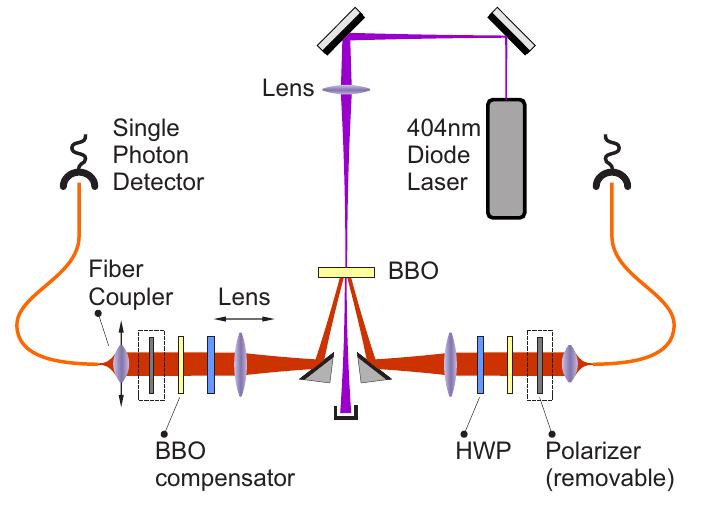
\includegraphics[width=.9\textwidth]{img/setup}
\caption{Schematic of the experiment setup. Image from \cite{skriptum}}\label{setup}
\end{figure}
In figure \ref{setup} the experiment setup is depicted. We used a blue laser source of 404 nm and 100 mW of power. With help of some mirrors this light is focused into a BBO crystal where SPDC happens and entangled photons are created. This process is purely quantum mechanical, one pump photon is converted into a photon pair, a signal photon with vertical polarization and a idler photon with horizontal polarization. Energy conservation in this process must hold and can be written as
\begin{equation}\hbar \nu_{pump} = \hbar \nu_{signal} + \hbar\nu_{idler},\end{equation}
this means that the sum of signal and idler frequencies must be equal to the frequency of the pump photon. Moreover, the photons must also obey momentum conservation
\begin{equation}\hbar \k_{pump} = \hbar \k_{signal} + \hbar\k_{idler}.\end{equation}
This implies that signal and idler photons are emitted in opposite direction with respect to pump photon, since wavevector must be conserved. Hence, entangled photons emerge in two different cones, and we can exploit this feature to split the beam in two separate arms of the setup, one for the horizontal polarized photons and the other for the vertical polarized ones. This is done in the experiment with two small prisms. Then each photon goes through a lens that collimate the beam into an halfwave plate for rotating the polarization by 90 degrees and after that inside another BBO crystal to compensate walk off effects. Walk off effects are due to the birefringence of the first BBO crystal where vertical polarized photon and horizontal polarized photon travel in different direction with different velocities. Therefore, entangled photon become distinguishable, so the second BBO crystal is used as compensation to restore indistinguishability. Before passing through the polarizer, photon are filtered in order to remove unwanted pump photons. Then, after the filter stage, there is a polarizer with a tunable angle. Finally photons are coupled inside optical fiber and measured with an avalanche photodiode (APD). APDs of both arm are connected together to a logical circuit which performs coincidence measurements. 

\section{Measurements and analysis}
\subsection{Visibility}
First of all, in order to test our setup we measured visibility in $HV$ base, with the following
\begin{equation}\label{eq:visibilityHV}V = \frac{N_{HV}+N_{VH}-N_{HH}-N_{VV}}{N_{HV}+N_{VH}+N_{HH}+N_{VV}},\end{equation}
where $N_{XY}$ is the number of coincidences when polarizer $A$ was set to $X$ and $B$ to $Y$. For every quantity we measured the number of coincidences over a time of one second for ten times, in order to have statistical error. Our measurement can be found in table \ref{tab:visibilityHV}, the error is the standard deviation. From this data we obtained $V = 0.94 \pm 0.08$,
Although the visibility is good (desired would be 1.0), there is a difference greater then 20\% between coincidence measurement of $HV$ and $VH$. This means that the setup is not properly aligned and it requires to be adjusted. Therefore, before proceeding in the next measurements, our supervisor aligned compensation crystals and checked visibility in the $DA$ base, which can be written in a similar way of \eqref{eq:visibilityHV}
\begin{equation}V = \frac{N_{DA}+N_{AD}-N_{DD}-N_{AA}}{N_{DA}+N_{AD}+N_{DD}+N_{AA}}.\end{equation}
Result in the $DA$ base can be found in table \ref{tab:visibilityDA}, where the measurements are done as for the $HV$ base and the error is calculated in the same way. We obtained a visibility of $V =  0.77\pm0.075$, which is worse then before, but now the coincidences of $DA$ and $AD$ are closer.
\begin{table}[h]
\centering
\begin{minipage}{.48\textwidth}
\centering
\begin{tabular}{c|c|c|c}
  & $A$& $B$& Coincidences \\
\hline
$HH$ & 90° & 90° & $0.4 \pm 0.15$\\
$VV$ & 0° & 0° & $0.2 \pm 0.13$\\
$HV$ & 90° & 0° & $5.2 \pm 0.5$ \\
$VH$ & 0° & 90° & $13.0\pm 0.9$\\
\end{tabular}
\caption{\label{tab:visibilityHV}Number of coincidences in $HV$ base, error on the angles is due to the resolution of the polarizers: 1°}
\end{minipage}\hspace{1.5em}% This must go next to `\end{minipage}`
\begin{minipage}{.48\textwidth}
\centering
\begin{tabular}{c|c|c|c}
  & $A$& $B$& Coincidences \\
\hline
$DD$ & 45° & 45° & $1.2 \pm 0.3$\\
$AA$ & 135° & 135° & $1.4 \pm 0.25$\\
$AD$ & 135° & 45° & $8.8 \pm 1.1$ \\
$DA$ & 45° & 135° & $11.7 \pm 0.7$\\
\end{tabular}
\caption{\label{tab:visibilityDA}Number of coincidences in $DA$ base, error on the angles is due to the resolution of the polarizers: 1°}
\end{minipage}
\end{table}
\subsection{Correlation measurements}
In order to measure the Bell's parameter, we did correlation measurements. First we set the polarizer $A$ at fixed angle 0° and then we measured coincidences at different angle of polarizer $B$. We went from 0° to 200° with a step of 4°, each time we took 1 second of coincidences for ten times in order to have statistics for the errors. We did the measurements again, but with the polarizer $A$ fixed at 45°. The plot of these two correlation measurements is in figure \ref{correlation}. The data has been fitted with a sine function of the form
\[C(\beta) = A\sin(\omega\beta +\phi) +  B,\] 
and yield as fit parameters to $A = 9.1\pm 0.2,\omega= 2.06\pm0.01\,[$°$]^{-1} ,\phi=-1.62\pm0.03,B=9.39\pm0.15$ for polarizer $A$ at 0° and $A = 5.5\pm 0.1,\omega= 2.10\pm0.02\,[$°$]^{-1} ,\phi=-2.67\pm 0.04,B=6.9\pm0.1$ for polarizer $A$ at 45°.
\begin{figure}[H]
\hspace{-5em}
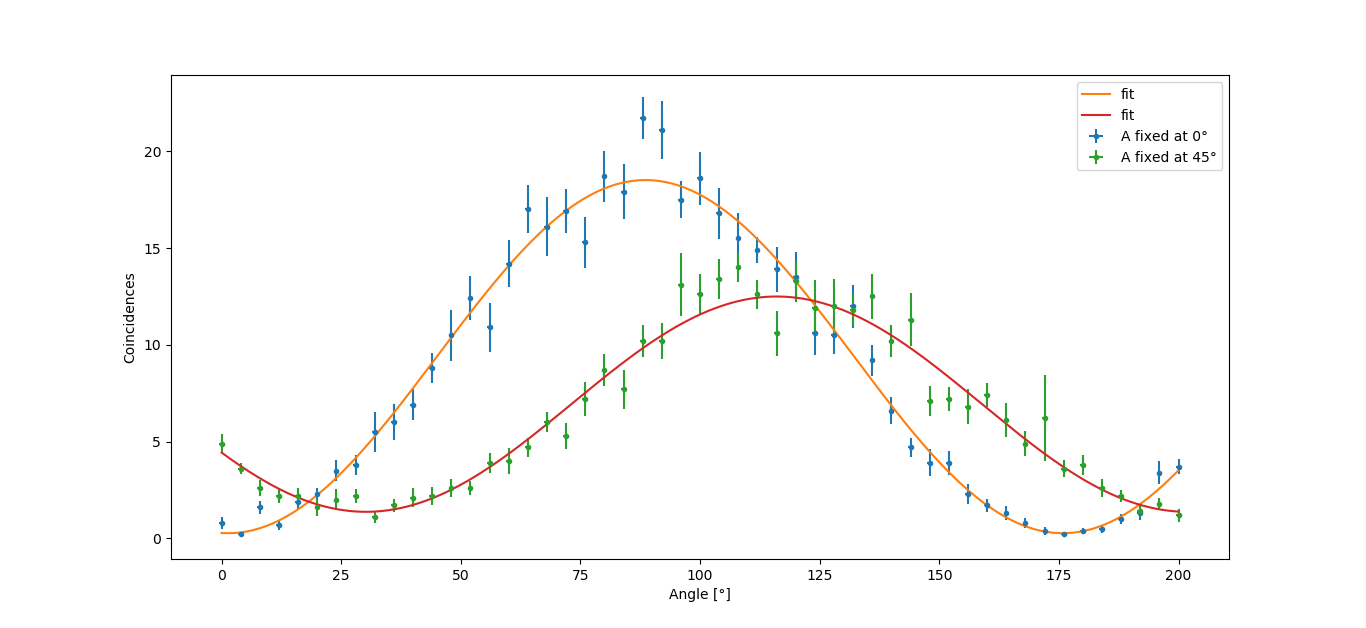
\includegraphics[width=1.2\textwidth]{img/correlation}
\caption{Correlation measurements, the error bars for the coincidences are based on the standard deviation of the mean over the ten measurements. The error of the angle is due to the resolution of the polarizer, and it is not visible because it is too small}\label{correlation}
\end{figure}
Unfortunately we did not have enough time to repeat the measurement for $\alpha = 45$° and $\alpha=135$°, so it is not possible for us to show the variation of the Bell's parameter as a function of $\beta$.
\section{Bell's parameter measure}
We performed extended measurements for coincidence, we took 100 different measure of coincidence for each pair of $\alpha,\beta$, each measure recorded one second of coincidences. The angles are chosen such as the Bell's parameter is maximized. The measurement can be found in table \ref{tab:extendedmeasures}, the error is the standard deviation of the mean over the one hundred measurements.
\begin{table}[H]
\centering
\begin{tabular}{c|c|c|c|c}
Angle  & $\alpha,\beta$& $\alpha,\beta+90$°&$\alpha+90$°$,\beta$& $\alpha+90$°$,\beta+90$° \\
\hline
$\alpha=0$°$,\beta=22.5$° & $3.14\pm0.17$ & $16.59\pm0.38$ & $7.42\pm0.27$ &$2.39\pm0.15$\\
$\alpha=0$°$,\beta=67.5$° & $17.63\pm0.44$ & $2.68\pm0.16$ & $1.37\pm0.11$ &$6.51\pm0.23$\\
$\alpha=45$°$,\beta=22.5$° & $2.43\pm0.16$ & $13.62\pm0.39$ & $8.39\pm0.31$ & $5.73\pm0.26$\\
$\alpha=45$°$,\beta=67.5$° & $5.44\pm0.25$ & $7.35\pm 0.30$ & $13.05\pm0.37$ & $1.09\pm0.12$\\
\end{tabular}
\caption{\label{tab:extendedmeasures}Result of the extended measurements}
\end{table}
Using equation \eqref{expectationvalue} and then equation \eqref{Bellinequalityi} we found a Bell's parameter of $S = 2.31\pm 0.04$, the error is calculated through error propagation. Our result is greater then two within the error, so Bell's inequality has been violated. \\
It is also possible to evaluate the visibility with this last result, in fact the visibility can be obtained as
\[V = \frac{S_{max}}{2\sqrt{2}}\]
in our case we obtained $V = 0.81 \pm 0.02$, which is in agreement within the error with the visibility reported before.
\section{Questions}
In this section we answer some preparation questions, as requested from our supervisor.
\begin{enumerate}
\setcounter{enumi}{3}
\item \textbf{Assuming a $\ket{\psi^-}$ i state, calculate explicitly the coincidence detection probability for linear
polarizer angles $\alpha$ and $\beta$}\\ 
We can write he state of a photon after passing through polarizer $A$ set at angle $\alpha$ as
\[\ket{\alpha}_A = \sin(\alpha) \ket{V}_A + \cos{\alpha}\ket{H}_A,\] 
similarly for the polarizer $B$ set at angle $\beta$ we have \[\ket{\beta}_B = \sin(\beta) \ket{V}_B+ \cos{\beta}\ket{H}_B.\]
If we assume an initial state equals to $\ket{\psi^-}$, the probability of a coincidence detection is
\[P = |\bra{\alpha}_A\bra{\beta}_B \ket{\psi^-}|^2 = \frac{1}{2}\sin^2(\alpha-\beta)\]
\item \textbf{The state of one of the photons, ignoring the other one is mathematically obtained by performing a partial trace, e.g. for photon $A, \rho_A = \mathrm{Tr}_B\{\rho_{AB}\}$, where $\mathrm{Tr}\{\}$ and the (partial) trace is linear. Calculate $\rho_A$ for $\rho_{AB} = \ket{\psi^-}\ket{\psi^-}$. What is the meaning of the state (density matrix) that you obtain? Try to re-express the result in the AD basis!}\\
We can calculate explicitly $\rho_{AB}$ with the definition of $\ket{\psi^-}$:
\[\rho_{AB} = \frac{1}{2}(\ket{H}_A\ket{V}_B - \ket{V}_A\ket{H}_B)(\bra{H}_A\bra{V}_B - \bra{V}_A\bra{H}_B) = \]\[\frac{1}{2}(\ket{H}_A\bra{H}_A \otimes \ket{V}_B\bra{V}_B +\ket{H}_A\bra{V}_A \otimes \ket{V}_B\bra{H}_B)-\ket{V}_A\bra{H}_A \otimes \ket{H}_B\bra{V}_B + \ket{V}_A\bra{V}_A \otimes \ket{H}_B\bra{H}_B ).\]
We can perform now the partial trace over $B$, the part regarding the system $A$ can be pulled out the trace and we only need to calculate the trace for the system $B$. The second and the third terms are 0, in fact
\[\text{Tr}_B(\ket{H}_B\bra{V}_B) = \text{Tr}_B(\ket{V}_B\bra{H}_B) = 0. \]
Therefore we obtain
\[\rho_A = \text{Tr}_B(\rho_{AB}) = \frac{1}{2}(\ket{H}_A \bra{H}_A +\ket{V}_A \bra{V}_A )\]
which is a mixed state of the states $\ket{H}$ and $\ket{V}$ with equal probability $1/2$. We can express this result in the basis $AD$ instead f $HV$ by using the transformation
\[\ket{V} = M \ket{A} \qquad \ket{H} = M \ket{D},\]
where $M$ is the following matrix
\[M = \frac{1}{\sqrt{2}}\begin{pmatrix}
  1 & 1  \\
  1 & -1
 \end{pmatrix}.\]
 We obtain:
 \[\rho_A = \frac{1}{2}(\ket{D}_A \bra{D}_A +\ket{A}_A \bra{A}_A),\]
since $M$ is unitary. This result can be also directly obtained by looking at the form of $\ket{\psi^-}$, in the basis $AD$ it keeps the same form of the representation in the basis $HV$, so the result must have the same form.
\item \textbf{Can anything interacting with photon $B$ change the reduced state of photon $A$? Discuss this question in the light of the result obtained for the previous question. What can you conclude about using entanglement for communication?}\\
As can be seen from the previous answer, the form of the state of system $B$ is significant for the result. Indeed, the trace on $B$ can delete or not some terms in the expression for $\rho_A$. Therefore, interaction with the state $B$ can change the state of $A$. This feature can be exploited in quantum information for building a secure channel of communication. If you send a photon and it gets intercepted, you will notice a change in the state of your photon. Hence, you are able to tell if your message was transmitted securely or not.
\end{enumerate}

 \begin{thebibliography}{99}

  \bibitem{bellpaper}
     \textsc{J. Bell}, \textit{On the Einstein Podolsky Rosen paradox}, Physics, 1 (1964), pp. 195–200.

  \bibitem{inequality}
   \textsc{J. F. Clauser, M. A. Horne, A. Shimony und R. A. Holt}, \textit{Proposed experiment to
test local hidden-variable theories}, Phys. Rev. Lett., 23 (1969), pp. 880–884.

\bibitem{skriptum}
Fortgeschrittenenpraktikum 2, \textit{Entanglement and Bell’s inequality}. \textsc{Gregor Weihs, Kaisa Laiho, Harishankar Jayakumar}. WS 2015/16
\end{thebibliography}
\end{document}
